%%%%%%%%%%%%%%%%%%%%%%

\chapter{Person Following}
\label{chapter:person_following}

There are many scenarios in which a person following robot could be useful. For example, a robot can carry luggage of travelers in airports, or groceries in a supermarket. Person following is also the enabling capability for interactive label acquisition during the \textit{Tour Scenario} discussed in Section \ref{sec:tour_scenario}. For the tour scenario, the robot needs to know how to follow a person before building an environment representation and providing services to the user.  There are two properties that a person following robot should have: robustness and social awareness. Typically, a service robot operates in a dynamic and populated environment, therefore the robot must be able to keep track of a single person even when they are temporarily occluded. Multimodal person tracking that is presented in Chapter \ref{chapter:multimodal_person_detection_and_tracking} helps the robot to have an estimate of the user's position. For the person following task, the robot has to track a designated user, and the detection thresholds of detectors are relaxed for robust tracking at the expense of more false positive detections. 

For intelligent following, the robot not only has to keep appropriate distance to the user, but also has to recognize $what$ the user is trying to do. For example, during the tour scenario, when the user stops, the robot should predict when the user is going to annotate a landmark, and it should come beside the user instead of standing behind. Moreover, the robot should be smarter when passing doors or following a person who is cutting a corner. In order to be able to handle these scenarios, the robot should act beyond purely reactive following behavior. It is desirable for the robot to anticipate what the user is going to do and take appropriate action. The current chapter will discuss the basic following behavior whereas Chapter \ref{chapter:following_situation_aware} will discuss situation awareness and improved behavior for person following.

In this chapter, after referring previous works on person following robots in Section \ref{sec:following_related_work}, we present a basic person following method in \ref{sec:following_basic_person_following}. In Section \ref{sec:following_application_to_telepresence}, we present an application of person following for telepresence robots.

\section{Related Work}
\label{sec:following_related_work}

A robot that follows a person is a widely studied scenario in robotics. A relevant body of work is pursuit evasion \cite{chung2011search}, in which the target is trying to evade the follower. In our applications, we assume that the target user is cooperating with the robot.

In one of the earliest works in this area by Sidenbladh \cite{sidenbladh1999person}, robot keeps the person centered in the camera image using a P controller. Prassler \cite{prassler2001motion} also offers a reactive approach using the \textit{Velocity Obstacles} concept, which uses the velocity of the target to find allowable velocities of the robot that guarantees avoiding collision if both the target and the robot moved with constant speed for future steps. The approach is applied on a wheelchair, however social constraints were not considered. Gockley \cite{gockley2007developing} observed how people walk together. It is reported that partners who were conversing tend to look forward with occasional glances to each other. Ohya \cite{ohya2002intelligent} presents a following method that escorts a target on the side while avoiding obstacles. It was assumed that the target would move with the same acceleration and velocity. Murakami \cite{murakami2014destination} presents a method to first estimate the sub-goal of the leading person and then following as if the robot knows the goal. Park \cite{park2013autonomous} models the problem as a control problem and offers an algorithm based on Model Predictive Control.
Miura \cite{miura2010development} employs randomized tree expansion and biases the calculated paths towards a sub-goal, which is the current position of the person. Hoeller \cite{hoeller2007accompanying} adopts the virtual targets idea and selects a goal position in a circular region around the person. Stein \cite{stein2013navigating} proposes choosing and following a leader to handle navigation in crowds.

Some of the relevant works considered the social side of the interaction. Gockley compared two elementary following methods in \cite{gockley2007natural}: direction following, where the robot always attempts to drive towards the tracked person, and path following, in which the robot follows the exact path the person took. It was shown that direction following behavior was perceived as more human-like and natural than path following. Yuan's approach \cite{yuan2008spatial} switches the following behavior between parallel, direction and path following depending on the layout of the obstacles. Zender \cite{zender2007human} emphasizes situation awareness for following and studies handling of doors and corridors. To handle the doors, the robot increases its following distance and that leads the robot to wait for a while. Following in a corridor is handled with an approach similar to Pacchierotti \cite{pacchierotti2005human}, and the robot's speed is adjusted. Loper \cite{loper2009mobile} presents a system that is capable of responding to verbal and non-verbal gestures and following a person. Granata \cite{granata2012framework} presents behaviors such as going towards, following and searching a user. Ota \cite{ota2013recovery} touches upon the recovery functions whenever the robot loses tracks of the leading person.

\section{Basic Person Following}
\label{sec:following_basic_person_following}

In this section, we describe our basic person following method, that is the default following mode. When the following behavior is initiated from a higher level process, first the guide person must be tracked. The robot looks for the closest person in the vicinity of the robot (within $2m$). If no person is detected for a period of time, then the command is invalidated. We use the approach described in Section \ref{chapter:multimodal_person_detection_and_tracking} to detect and track users.

\begin{figure}[ht!]
\hspace*{4cm} 
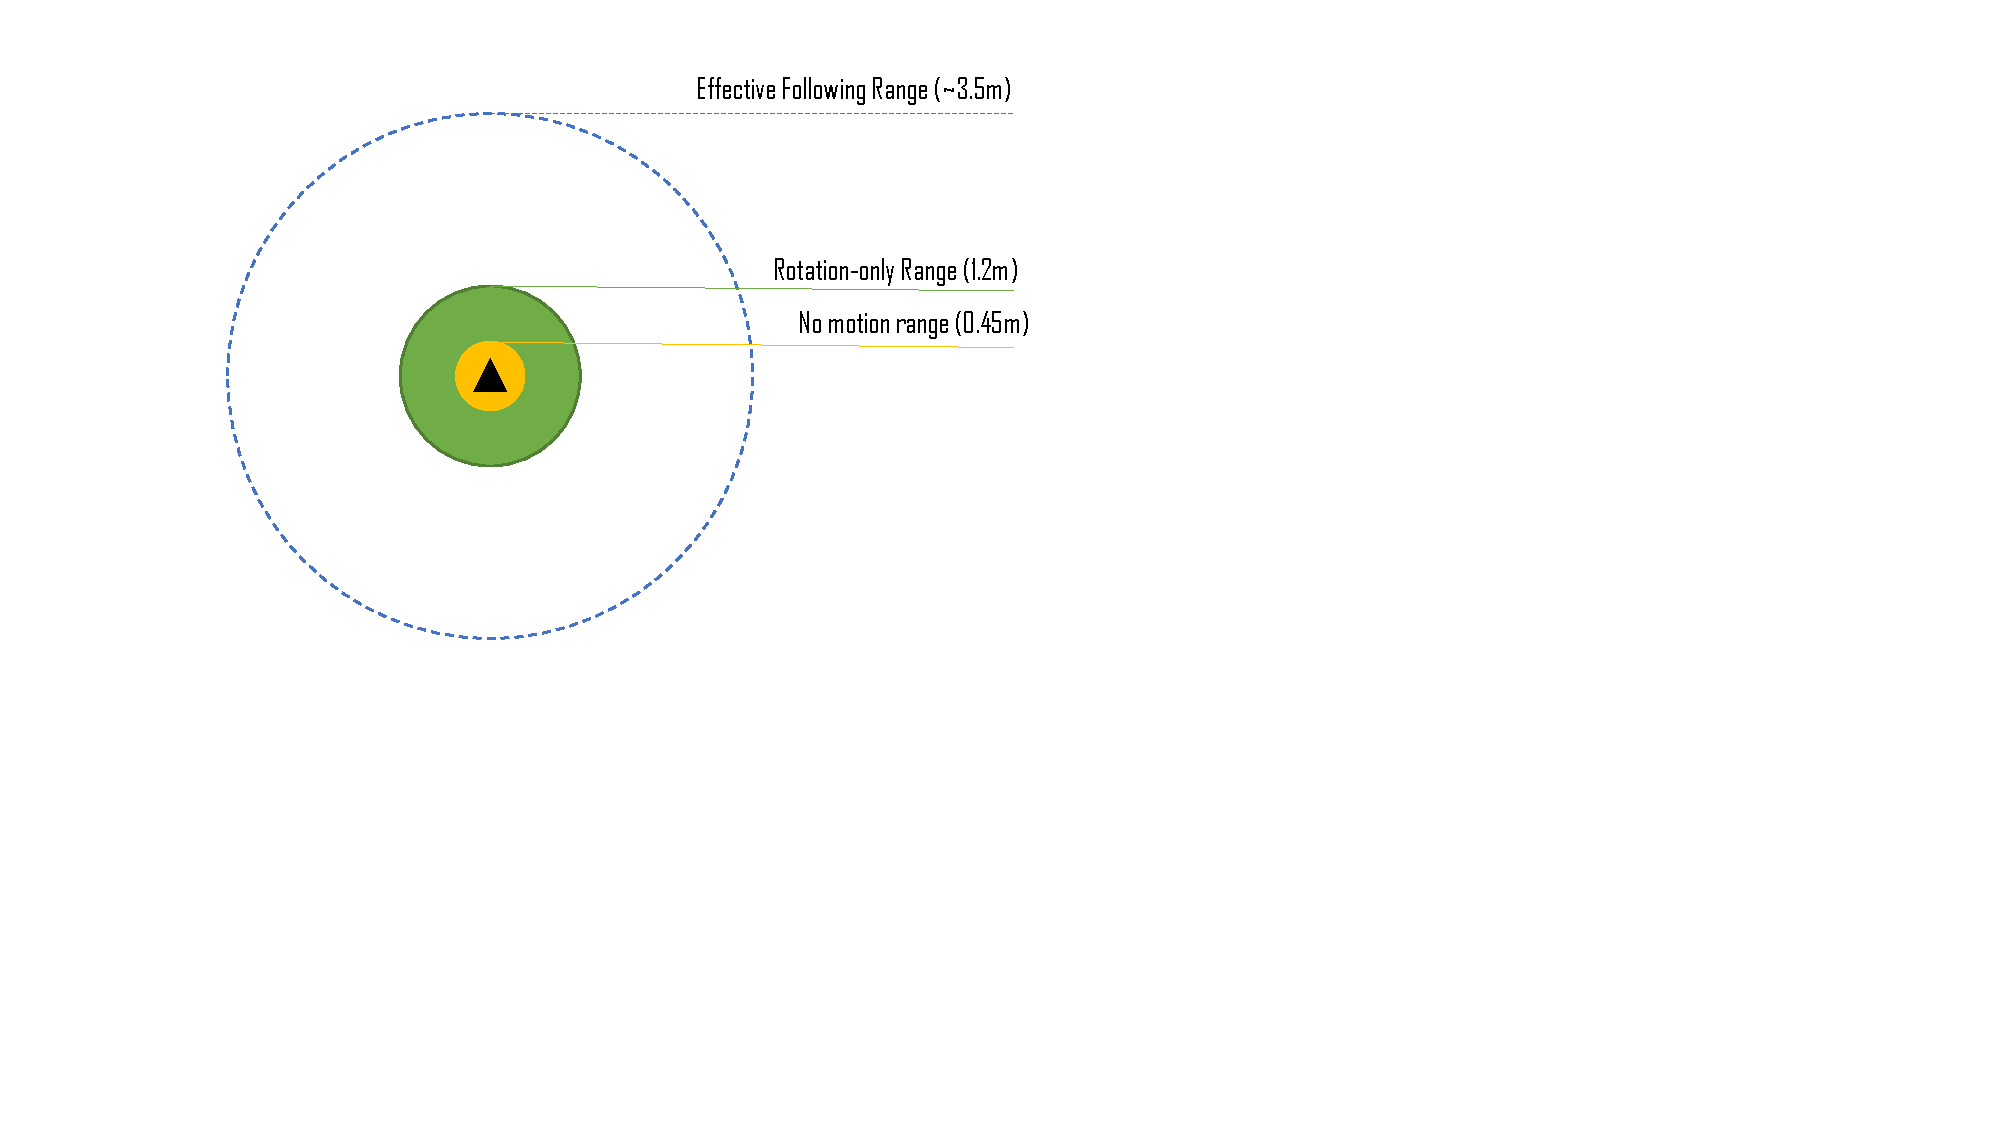
\includegraphics[width=0.65\textwidth]{pics/following_ranges_cropped}
\caption{Overhead sketch of the robot and relevant ranges for person following. Robot is represented as the triangle in the middle.}
\label{fig:following_ranges}
\end{figure}

In the basic person following mode, the robot has three different strategies depending on the distance towards the followed person. The distance to the user is calculated as the distance from the center of the robot base to the person's current location estimation. We used Hall's characterization of personal spaces in order to determine the distance limits. The three distinct zones and corresponding robot behavior are defined in Hall's work \cite{hall1969hidden} as follows:

\textbf{Intimate Zone $[0-0.45m]$:} The person is very close to the robot, therefore any motion of the robot may be potentially unsafe. The robot comes to a complete halt in this zone ($v=0,w=0$). A full stop also allows the user to safely interact with the on-board tablet GUI.

\textbf{Personal Zone $[0.45-1.2m]$:} When the robot is in the personal zone of the user, the robot stops and rotates towards the followed person ($v=0,w=w_{rotation}$). The rotational velocity is determined with a P controller, with the error term defined as the difference between the robot's current orientation and the tracked person's orientation. The rotational speed is capped at a fixed value, so that the person feels comfortable with the rotation speed of the robot.

\textbf{Social Zone $[1.2m-3.5m]$: } In this range interval, the robot executes the main following behavior. At every time step, a goal pose that is $1.2m$ away from the and headed towards the user is calculated (see Figure \ref{fig:following_1m} for an illustration). A collision-free path is found and the robot executes this path until a new measurement from the target person is received. The path is found using Dynamic Window Approach (DWA) local planing method. We use the ROS implementation of DWA for the basic following behavior.

\begin{figure}[h!]
\centering
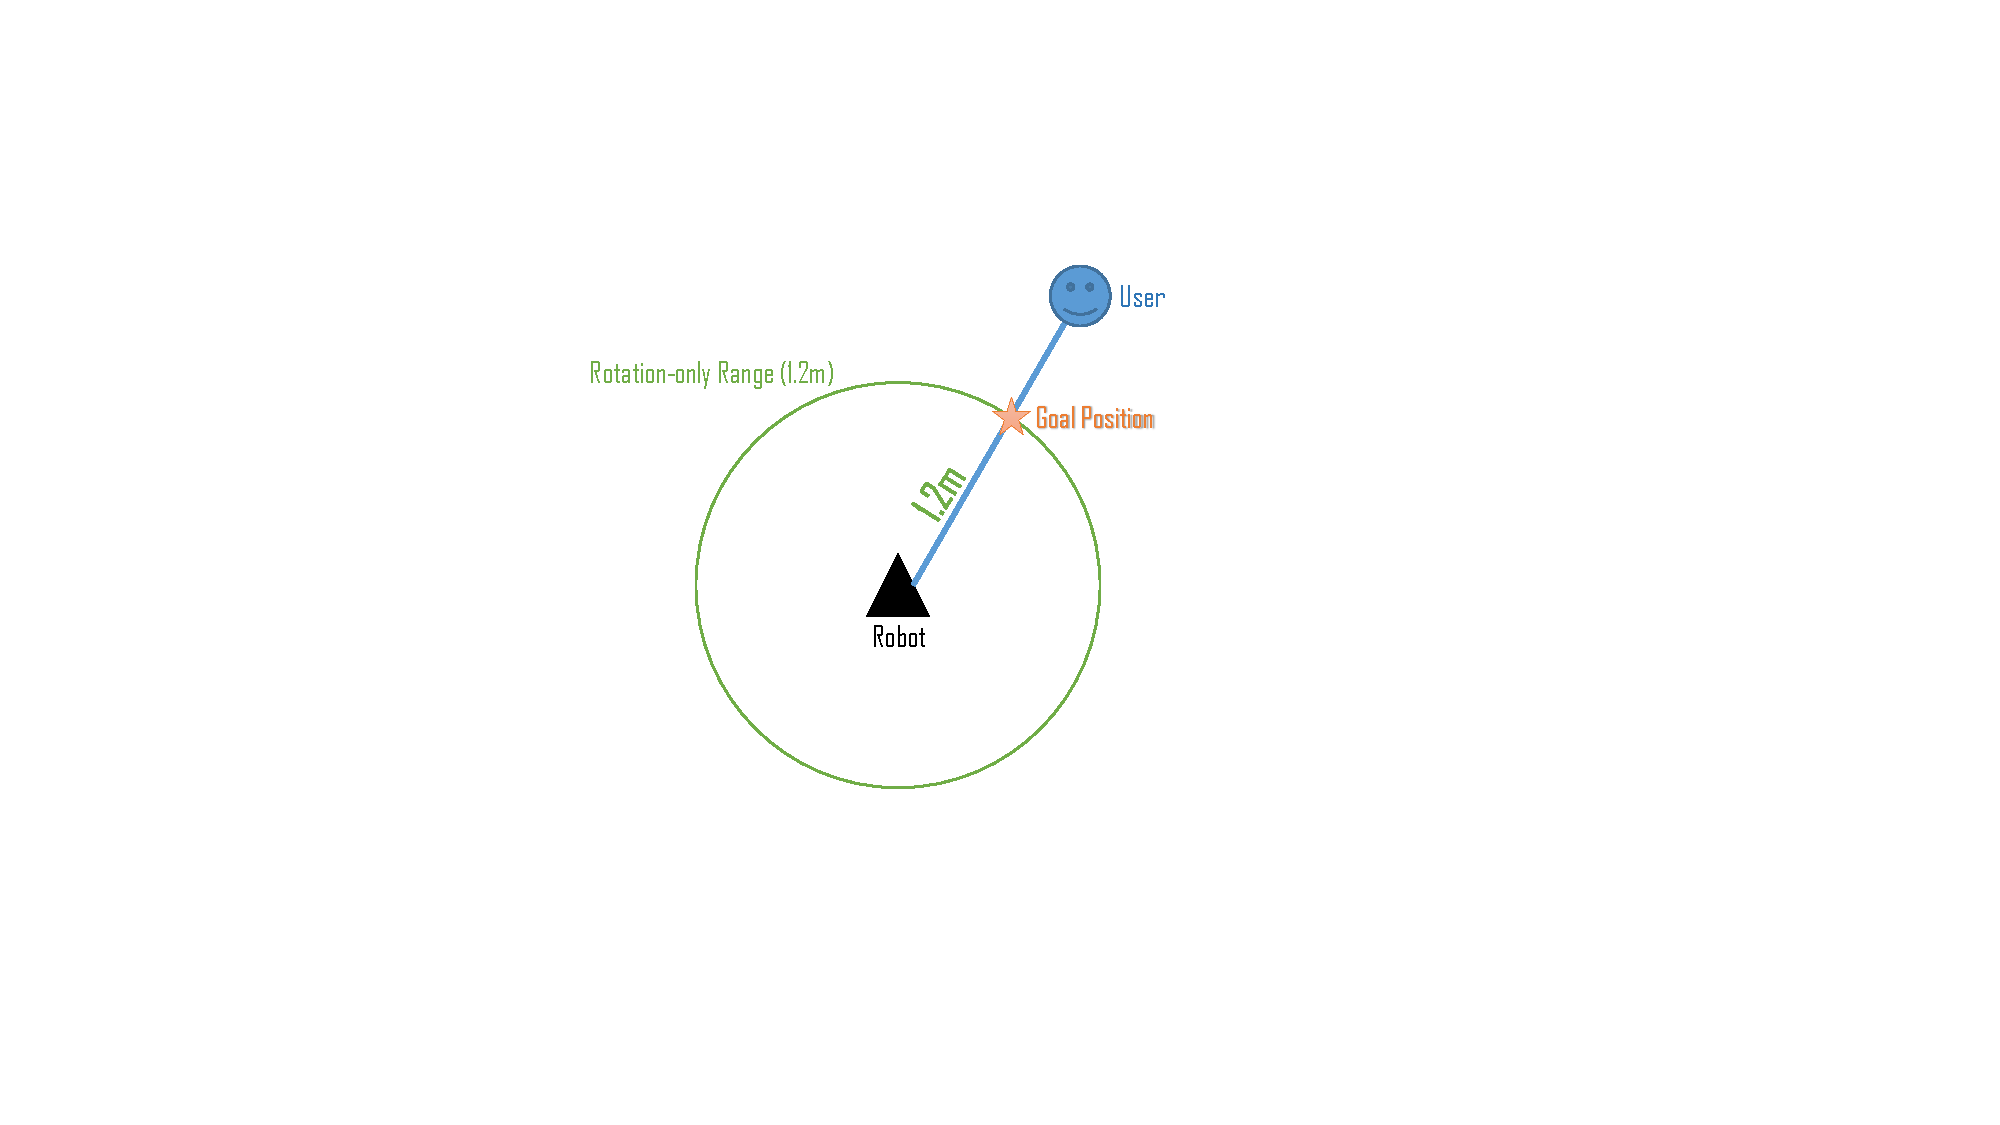
\includegraphics[width=0.55\textwidth]{pics/following_1m_cropped}
\caption{An illustration of how the goal position is calculated when the user is in the social space $[1.2m-3.5m]$.}
\label{fig:following_1m}
\end{figure}

Sometimes it is inevitable that the person tracking system loses the target, particularly when the person is consistently faster than the robot or the person goes outside the range of the sensors (further than $\sim3.5m$ in our case). When this happens, the robot will attempt to go to its last calculated goal position and look for the person. With this behavior, the robot attempts to keep up with the lost person as far as possible with the hope that the person will re-appear in the vicinity of the last seen position. After the robot reaches this goal, it stops and waits for an amount of time. If the user is saved to the database, or the robot already knows that he/she is in the database, then the face recognition system that will be described in Section \ref{sec:multimodal_face_recognition} is activated. Otherwise, the robot continues following the closest person that appears in this position. If no person is detected within a fixed amount of time ($5$ seconds in our implementation), then the robot declares that the person is lost and starts listening for a new following command.

\section{Application To Telepresence Robots}
\label{sec:following_application_to_telepresence}

A telepresence robot can be described as \textit{Skype on wheels}, where a remote user teleconferences in a physical environment while having the motion control of a robotic system. Telepresence robots constitute a promising area in the consumer robotics industry as evidenced by recent start-up companies working on telepresence products. However, currently all the telepresence robots that are available in the market are controlled by manual driving by the remote controller - usually via the keyboard or a joystick. In this section, we present an implementation of person following on a telepresence robot and a user study that evaluates effect of having person following capability on a telepresence robot.

Telepresence robots are a level above video conferencing since the robot is used as the communication medium and the remote user can now control the movement. Therefore, the spatial interaction between people and a telepresence robot in social situations is worth investigating. One of those situations is moving with a group of people. In an effort to analyze the spatial and verbal interaction, we focus on engagement with one person where the remote user interacts with the person while following him/her in a corridor. This is situation is very likely to happen in office environments, for example when the remote user is having a discussion with a co-worker while walking to his office after a meeting. As telepresence robots become more common, there will be need to have the functionality of autonomous following of a person so that the remote user doesn't have to worry about controlling the robot.

We evaluate our system by conducting a user study, where there are two following conditions:

\begin{enumerate}
\item Manual Person Following: Robot is controlled with an Xbox controller
\item Autonomous Person Following: Following is initiated by clicking on a user in RGB-D image
\end{enumerate}

The aim of the user study is to measure how remote users like using the autonomous following feature compared to the manual. For the study, the remote user has a task that consists of listening to a passage the guiding person reads, and answering related questions after the interaction. We also observe subjects' experiences using the system, get useful feedback to pinpoint future challenges that can be helpful designing new generations of telepresence robots.

\subsection{Robot Platform}

\begin{figure}[h!]
\centering
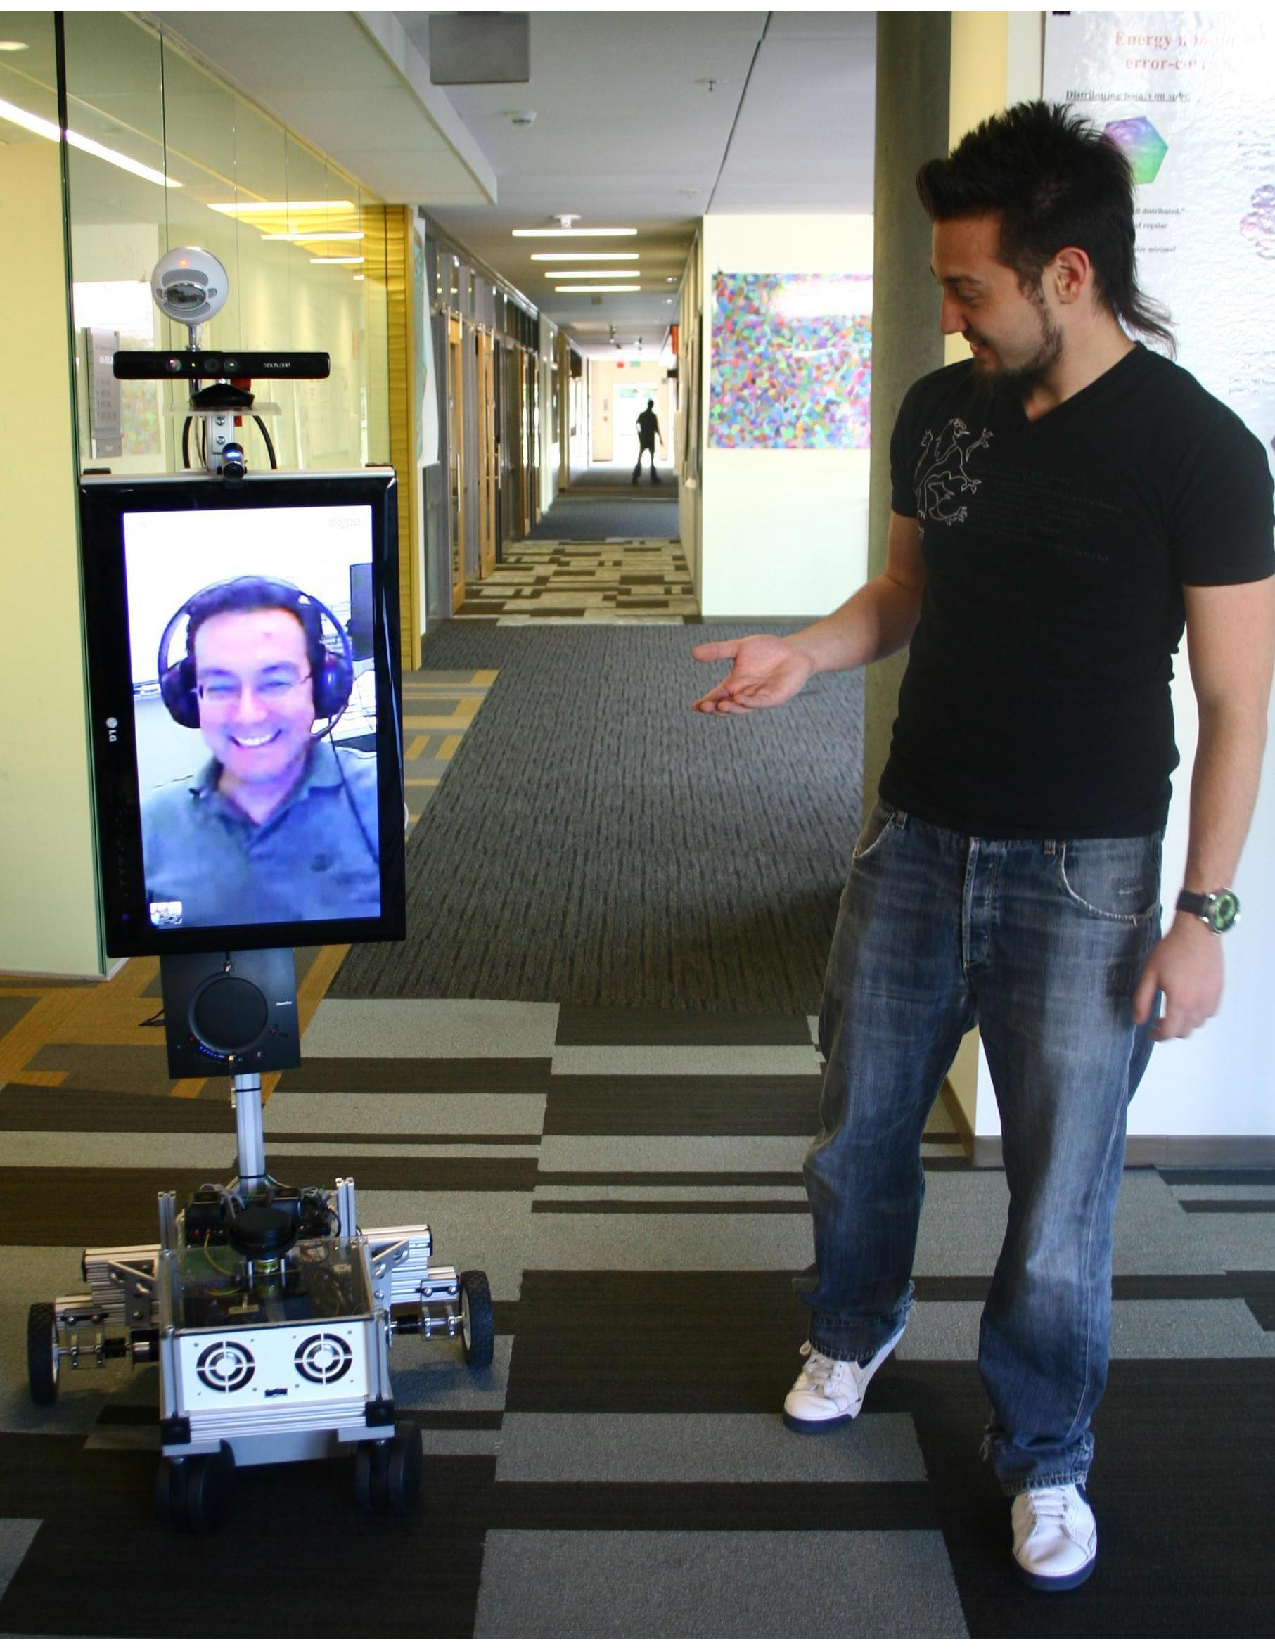
\includegraphics[width=0.4\textwidth]{pics/telepresence_robot}
\caption{The telepresence robot platform we used for our experiments.}
\label{fig:telepresence_robot}
\end{figure}

The system described in this paper is implemented on an experimental telepresence robot platform shown in Figure~\ref{fig:telepresence_robot}. The robot has a differential drive base and can be used for about 8 hours with full charge. The remote user connects to the robot via wireless internet and communicates with others using Skype. The robot is also equipped with an omni-directional microphone and a high-end speakerphone. A wide-angle camera is placed on top of the monitor and tilted slightly downward to help the remote user to see the floor, robot base and people's faces at the same time. A Kinect Sensor is also placed above the monitor. Person following is initiated using the user interface shown in Figure \ref{fig:telepresence_ui}.

\begin{figure}[h!]
\centering
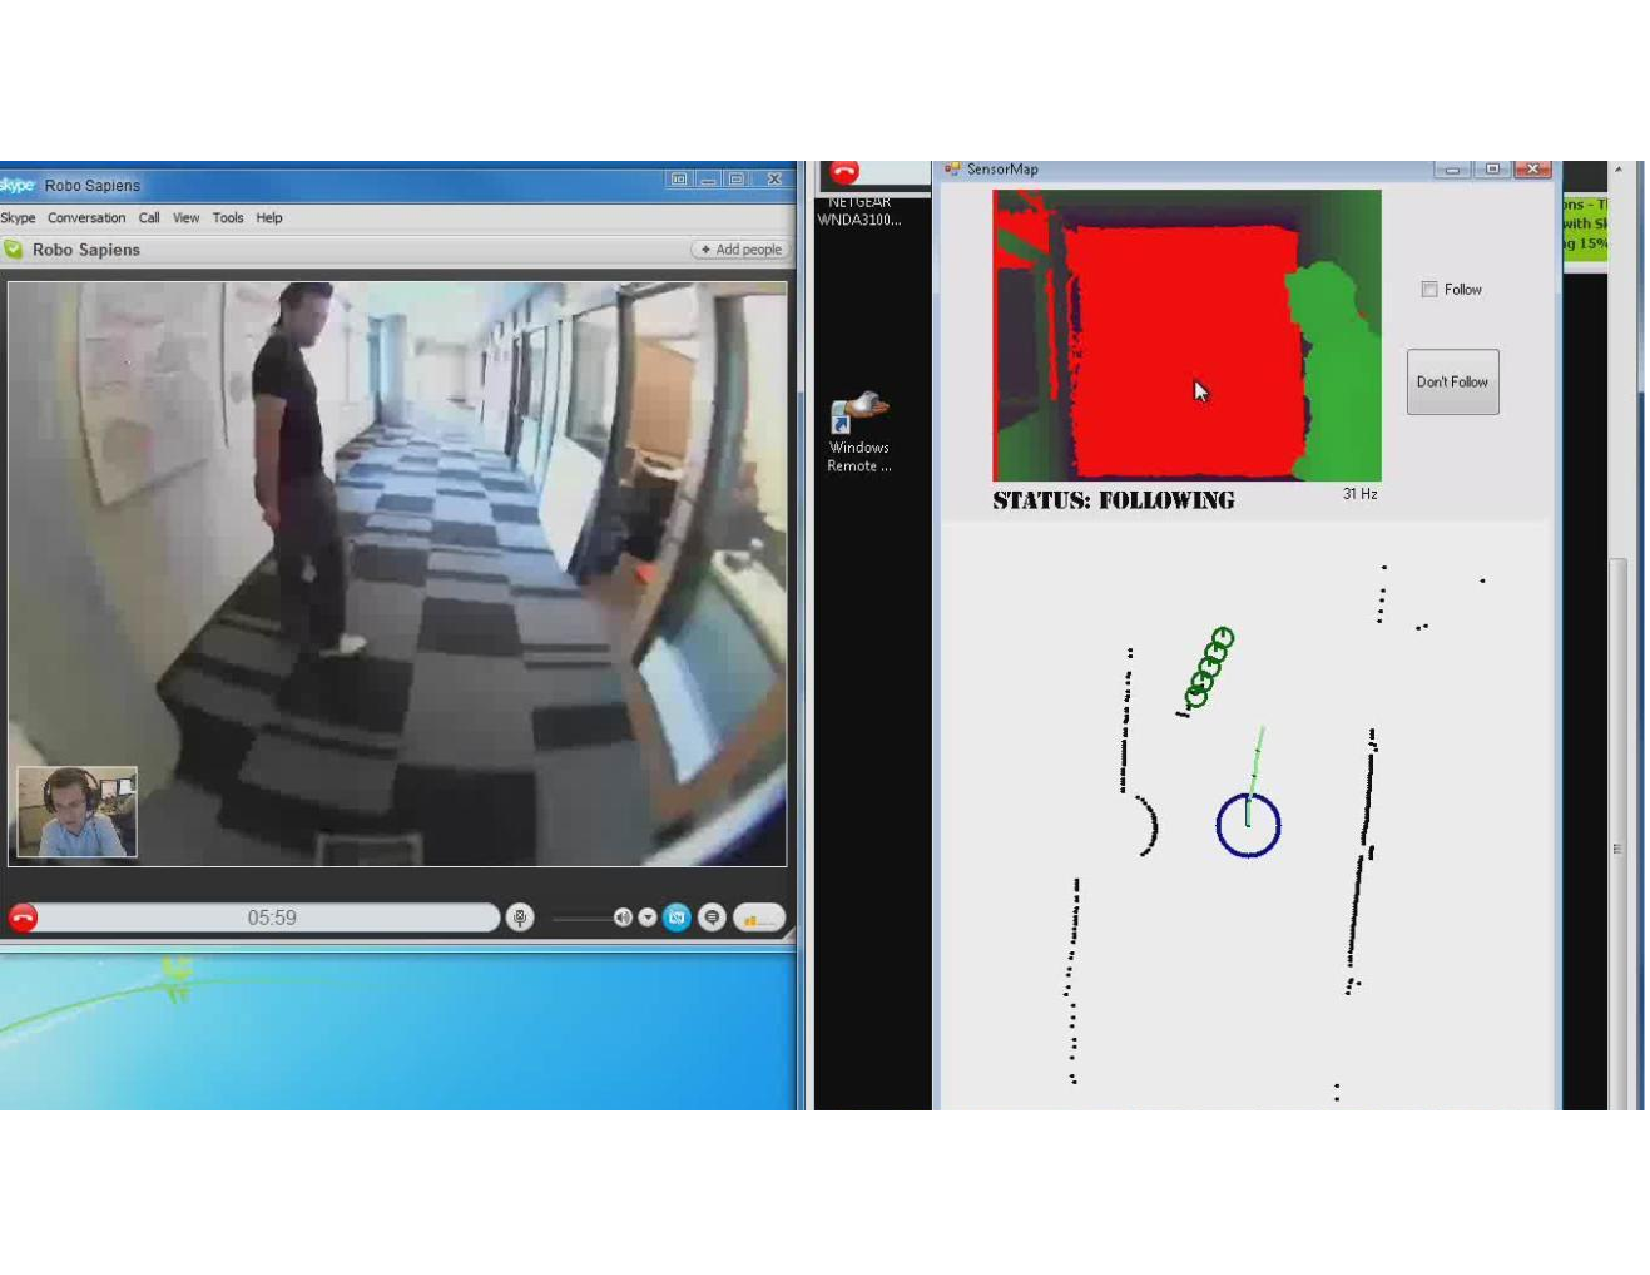
\includegraphics[width=1.0\textwidth]{pics/telepresence_ui_cropped}
\caption{User Interface of the robot for the remote user.}
\label{fig:telepresence_ui}
\end{figure}

A modified version of the local planner used in Section \ref{sec:navigation_local_planner} is used for person following. A utility function consisting multiple factors, including the respective position to the person, is optimized over multiple steps using Breadth-First Search. Details of this path planning method can be found in \cite{cosgun2013autonomous}.

\subsection{User Study}

In this study, remote user is the subject and the followed person is the experimenter. To investigate the effectiveness of using autonomous person following for an interaction task, we ran a controlled experiment and varied manual vs. autonomous following within subjects.

\paragraph{Design:}
The experiments were conducted in working hours and bypassers were free to walk across the experiment area or talk. The subjects were given the task of following the experimenter through the course for a lap and listen to the passage he is reading. In the first run, the subject used one of the autonomous following or teleoperation methods to follow a person and complete the lap. In the second run, the subject used the other method. At the end of each run, the subject was asked to complete a 4-question quiz about the passage. At the end of both runs, the user was asked which method he/she will prefer over the other for this type of a scenario. The exact questionnaire can be found in Appendix \ref{chapter:telepresence_user_study_survey_questions}. The passages and quiz questions were taken from Test of English as a Foreign Language (TOEFL) listening section examples. The passages were chosen so that they are at a similar difficulty level. The time it takes to read a passage corresponded approximately to the same time a lap is completed. We also asked numbered 7 point Likert scale questions, administered after each run, about how \emph{Understandable} the experimenter was, if the UI was \emph{Easy to Use}, if the robot exhibited \emph {Natural Motions}, how \emph{Safe} the remote user felt, if the subject was able to \emph{Pay Attention} to the passage, how \emph{Fast} the robot was and how much \emph{Fun} the subject had.

\paragraph{Participants:}

10 volunteers participated in the study (6 male and 4 female between the ages of 25-48). 5 of the participants had little knowledge, 4 had average knowledge and 1 had above average knowledge on robotics. The participants weren't gamers: 4 participants never played console games, 4 played rarely, 1 sometimes played and 1 often played. 6 of the participants often used video conferencing software, while 2 sometimes and 2 rarely used. 9 of the participants were not native English speakers and all of them had taken the TOEFL before.

\paragraph{Procedure:}

The participants were first greeted by the experimenter and instructed to complete a pre-task questionnaire regarding their background. The robot was shown to the participant and basic information about its capabilities was told. The experimenter explained the task while walking with the participant in the experiment area and showing the course to be followed. Participants were told that they should stay close to the experimenter while he is walking and there will be a quiz regarding the passage afterwards. The participant was informed that there are 2 operation modes: manual and autonomous person following.

Before the experiment started, the participant went through training for about 15 minutes. First, the participant learned the basic controls for the Xbox controller when he/she was nearby the robot. Then the participant was taken to the remote station, which was about 20 meters away from the corridor area. The participant was informed about the UI and was shown how the autonomous following is activated. Then a test run was executed, where the remote user followed the experimenter via teleoperation and had a conversation.

After the training, the actual run was executed using one of the manual or autonomous methods. We switched the starting method for every other experiment in order not to bias the subjects' opinions about one particular method. When the lap was completed, first the passage quiz, then the survey questions were answered by the subject. Then, the second experiment using the other method was executed and the second passage quiz and survey questions were given to the subject. As the last question, the subject was asked to state his/her method of preference. Lastly, the participants were debriefed about the study and engaged in a discussion. 

\paragraph{Measures:}
We had three measurement criteria to compare manual vs autonomous following: 

\begin{enumerate}
\item  Number of correct answers to passage quizzes: Assuming the standardized TOEFL exercises were of same difficulty, we ran a paired $t-test$ on two groups of autonomous and manual.
\item Survey questions: We ran a paired $t-test$ using 7-point Likert Scale on each of the seven questions.
\item Preferred Method: We looked at which method subjects chose over the other one.
\end{enumerate}

\paragraph{Results:}

Out of the 4 quiz questions, the correct answers for autonomous group ($\mu=2.9$, $\sigma=0.9$) were more than the manual group ($\mu=2.2$, $\sigma=1.2$) but the statistical difference was not statistically significant ($t(9)=1.48$, $p=0.17$ on $t-test$).

Table \ref{table:telepresence_table} summarizes the survey results. For \emph{Understandable} and \emph{Fun}, the scores slightly favored autonomous method but the difference wasn't statistically significant. Manual method was found to be easy to use ($\mu=5.0$, $\sigma=2.2$), but the UI for autonomous method (clicking) was found to be marginally easier ($\mu=6.5$, $\sigma=0.9$), ($t(9)=2.13$, $p=0.06$). The motions of the robot was found to be significantly more \emph{Natural} to have a conversation for autonomous method ($\mu=5.4$, $\sigma=1.0$) than manual method ($\mu=3.5$, $\sigma=1.9$), ($t(9)=2.52$, $p=0.03$). Participants thought they were able to \emph{Pay more Attention} to the passage the experimenter is reading when the robot was following the him autonomously ($\mu=5.3$, $\sigma=1.8$) compared to manual method ($\mu=3.4$, $\sigma=1.5$) and the statistical difference was significant ($t(9)=2.63$, $p=0.02$). Participants have found the autonomous method ($\mu=5.1$, $\sigma=1.7$) safer than manual method ($\mu=2.3$, $\sigma=1.4$) and there was a significant difference between two groups ($t(9)=3.09$, $p=0.01$). The speed of the robot was found to be neither fast nor slow for both methods ($\mu=3.9$, $\sigma=0.3$) and ($\mu=4.3$, $\sigma=0.8$).

All 10 subjects chose autonomous person following over teleoperation for this task.

\begin{table}

	      \caption{Survey results of the user study for person following for telepresence robots. Table displays survey question average and standard deviations for the two conditions: Autonomous Person Following and Manual Person Following.}
	      	\centering
  \begin{tabular}{lSSSSSS}    
  \toprule
    \multirow{2}{*}{Question} &
      \multicolumn{2}{c}{Autonomous} &
      \multicolumn{2}{c}{Manual Drive} &
      \multicolumn{2}{c}{$t-test$} \\
      & {$\mu$} & {$\sigma$} & {$\mu$} & {$\sigma$} & {$p$} & {$t$} \\
      \midrule
    1. Understandable & 4.0&	1.5&	3.6&	1.7&	0.47 & 0.73 \\
    2. Easy UI & 6.5&	0.9&	5.0&2.2&0.06& 2.13 \\
    3. Natural Motion &  5.4 & 1.0& 3.5 & 1.9 & 0.03 & 2.52 \\
    4. Safe & 5.1 & 1.7 & 2.3 & 1.4 & 0.01 & 3.09 \\
    5. Pay Attention & 5.3 & 1.8 & 3.4 & 1.5 & 0.02 & 2.63 \\
    6. Fast & 3.9 & 0.3 & 4.3 & 0.8 & 0.10 & -1.8 \\
    7. Fun & 5.3 & 1.5 & 5.1 & 1.7 & 0.66 & 0.45 \\
    \bottomrule
  \end{tabular}
    \label{table:telepresence_table}
\end{table}


\subsection{Design Implications}

Our user study showed that a person following behavior is desirable for telepresence robots when there is interaction. The follow-up discussions also agreed with the survey results, as one subject (R10) stated: \emph{``It just gives me more focus and concentration.''} Below, we list our observations and implications for future research and design for telepresence robots:

\textbf{Motor Noise:} Even though the motors on the robot were relatively quiet, 8 out of 10 participants expressed that the motor noise made communication harder. This justifies the close scores we collected in the survey question asking if the subject was able to understand what the experimenter was saying. (R8) was disturbed by the noise: \emph{``When I was driving, it was always this constant sound. It was worse for the autonomous one. It was constantly adjusting and compensating for the movement."} On the other hand, (R5) found the motor noise useful: \emph{``I actually like it because it gives me the feedback whether I'm driving faster or slower. It also gives me a little bit feeling of life."} Thus, although excessive motor noise should be avoided, some noise might be useful.

\textbf{Wireless Connection:} Second most cited problem for video conferencing was the video quality and time lags. (R8) clearly expressed why it was hard to walk with the experimenter using the manual method: \emph{``The frame rate drops all of a sudden and you have no choice but to stop."} Another subject (R9) made use of the displayed sensor data when the video conferencing quality went bad: \emph{``Because of the lag, I just switched to the Kinect (depth image) and the overhead view (laser)."} This was possible because the wide angle camera image was coming from Skype whereas sensor displays were received from the Windows Remote Assistance. Clearly, a big challenge for telepresence systems is to deal with wireless connection problems.

\textbf{Natural Interaction:} Even though the participants thought the motions of the robot were natural to have a conversation ($\mu=5.4$, $\sigma=1.0$), some didn't feel it was a natural way to communicate. As seen in Figure \ref{fig:telepresence_robot}, the screen displaying the remote user's face is flat and it introduced problems when the robot was traveling side-by-side to the person. (R5), when asked about walking side by side: \emph{``..we don't have face-to-face. It is not really a conversation."} This raises design considerations on how the remote user's face is brought out. One of the subjects (R5) discovered that the microphone characteristics are different than human hearing: \emph{``I don't have a distance sense if the experimenter is further away or close. If you have the fading audio, then I'll immediately notice."} Whether a telepresence robot should exhibit the same characteristics of human perception or not is an open question and needs further investigation.

\textbf{Assisted Teleoperation:} Telepresence robots should possess a layer to assists the remote user to avoid obstacles and collisions. \emph{Safety} ratings for the manual method were very low ($\mu=2.3$, $\sigma=1.4$) and (R8) expressed the concern: \emph{``I was especially worried about running into the experimenter."} This suggests that scenarios involving interaction would demand more attention of the remote users. The teleoperation should also be intuitive and be similar to driving modalities that people are already used to. (R4) stated: \emph{``I was thinking about Manual mode compared to driving a car."} before suggesting \emph{``.. maybe something like a cruise control might be good."}

\textbf{Gaming Experience:} Since the robot was controlled by a gaming console controller, some participants likened the manual mode to gaming. (R9) said: \emph{``Manual is like playing video games."} and (R5) said: \emph{``I don't play video games so controlling those consoles is not natural to me."} Thus, it is possible that gamers are less likely to have trouble driving the robot. The same observation was made by Takayama \cite{takayama2011assisted}.

\textbf{Long Term Interaction:} None of the subjects who participated in our study had used a telepresence robot before. (R6) justified the inability to use the manual method: \emph{``Maybe if I have some more practice for about several hours of driving the robot, I can use manual as well as autonomous.''} (R8) on having fun using teleoperation: \emph{``It was fun because it was the first time I did it but I can imagine that over time, I'll get bored of it."} The \emph{Fun} question in the survey received similar scores for autonomous and manual, possibly because using a telepresence robot was a new experience for the subjects. Studies regarding long term interaction for telepresence robots can yield interesting results, as in \cite{lee2011now}.

\textbf{Error recovery:} When the person was lost during following, the UI displayed a text that the person was lost so that the remote user can re-initiate the following by clicking on the person. None of the subjects complained about the robot losing the person. When asked explicitly about the robot losing the experimenter, (R10) answered: \emph{``That's not a big deal in comparison to me driving the robot."} Therefore, applications developed for telepresence robots can take advantage of the human being in the loop and does not have to be error-free for deployment.

\subsection{Discussion}

User studies showed that autonomous person following
is a desired capability for telepresence robots and it was
favored over direct teleoperation for an accompanying task.
Autonomous following was found to be safer, easier to use
and helped the remote users to pay more attention to the
conversation instead of the robot control. From the experience
earned from user studies, there are still interesting
challenges to explore in terms of human-robot interaction for
telepresence robots.

%%%%%%%%%%%%%%%%%%%%%%